% GENERATED by haipipe-display scripts/build_preview.py: page 1 the display, pages 2+ how it was made. Rerun it.
\documentclass[12pt]{article}
\usepackage[letterpaper,margin=1in]{geometry}
\usepackage{fontspec}
\IfFontExistsTF{TeX Gyre Termes}{\setmainfont{TeX Gyre Termes}}{\IfFontExistsTF{Times New Roman}{\setmainfont{Times New Roman}}{}}
\usepackage{microtype}
\usepackage{graphicx,booktabs,tabularx,multirow,array,longtable,amsmath,amssymb,setspace,caption,float,xcolor}
\usepackage{fancyhdr}
\onehalfspacing
\setlength{\parindent}{0.25in}
\setlength{\parskip}{0.35em}
\pagestyle{fancy}\fancyhf{}
\renewcommand{\headrulewidth}{0pt}
\fancyfoot[C]{\thepage}
\usepackage{float}
\begin{document}
\makeatletter\renewcommand{\fps@figure}{H}\renewcommand{\fps@table}{H}\makeatother
\renewcommand{\figurename}{eFigure}\renewcommand{\tablename}{eTable}\renewcommand{\thefigure}{1}\renewcommand{\thetable}{1}
\begin{figure}
  \centering
  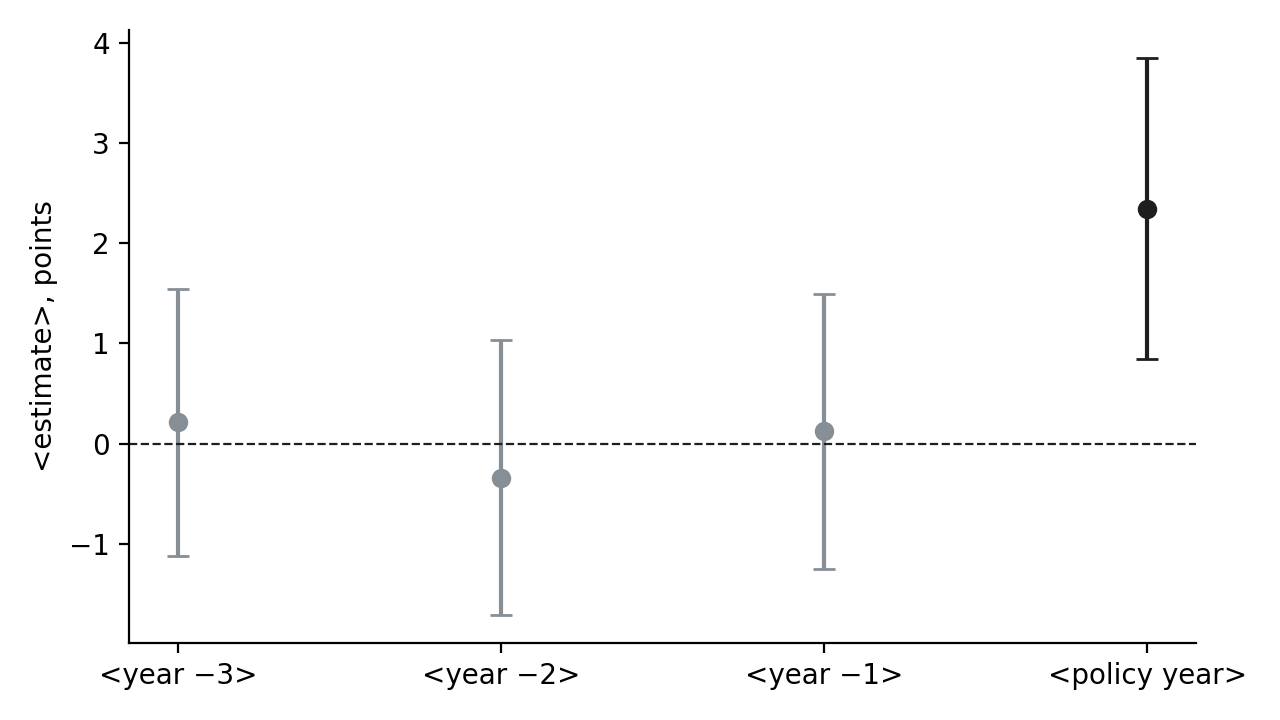
\includegraphics[width=\linewidth]{assets/figure.png}
  \caption{\textbf{<Placebo check>: the same model in years with no policy.} Points show each estimate with its 95\% interval; the dashed line marks zero; the last point is the policy year. Placeholder figure of Tools' Paper-Example; no real data.}
  \label{fig:placebo}
\end{figure}

\clearpage
\section*{What this display says}
In the years before <the policy> the same model finds no effect, so the effect in the policy year is not a trend that was already there.

\section*{How this display was made}
\subsection*{Data}
<The data source>, years <YYYY to YYYY>: the work Run b90.j02.t01.r01, its result/values.csv (placeholder).

\subsection*{Sample}
\begin{itemize}\item <who is in it>, as in Display A
\end{itemize}
\subsection*{Method}
The main model refitted with <the policy> moved to each earlier year, where it did not happen; each estimate with its 95\% interval. The placebo estimates are placeholders.

\subsection*{Made by}
\begin{itemize}\item \texttt{r01\_example\_main/result/values.csv} (the policy-year estimate: main.b, main.ci\_lo, main.ci\_hi), the Run of
\end{itemize}
\texttt{work/b90\_example\_paper\_results/j02\_example\_estimates/t01\_example\_main/}

\begin{itemize}\item \texttt{j01\_evidence\_display/t03\_display-c-placebo-check/scripts/draw\_placebo\_check.py}
\end{itemize}
\subsection*{Numbers}
The policy-year estimate is read from values.csv above; the placebo estimates are fixed placeholders.

\end{document}
